% \section{\centering \large CAPÍTULO 5}

\begin{justifying}
    Esta relación de precedencia es irreflexiva porque ningún evento propio se compone consigo mismo; es asimétrica: si dos eventos se componen en un orden dado, no se deduce que también se compongan en el orden inverso; y es transitiva: si un evento se compone con otro, y este último con un tercer evento, entonces el primero se compone con el último. En resumen, < es un orden parcial estricto de E(x) para cualquier cosa x. (La precedencia es entonces formalmente igual a < en un conjunto de números y a c en un conjunto de conjuntos). En resumen, tenemos
    
    \bigskip COROLARIO 5.5 Para cualquier cosa dada x y cada representación de estado,\bigskip $(E(x), <)$ es un conjunto estrictamente parcialmente ordenado.
    
    Que cada espacio de eventos esté ordenado por < significa que, siempre que dos eventos en él sean componibles, uno de ellos precede al otro. Este orden no está conectado: hay eventos en cada $E(x)$ que no se preceden ni se suceden entre sí, como lo demuestra la propia definición de la composición * de eventos como una operación parcial. Además, ese orden es relativo o dependiente del marco, en lugar de absoluto o invariante del marco, porque $E(x)$ en sí mismo es dependiente del marco. Por lo tanto, si e precede a e' en relación con un determinado marco, puede existir otro marco en relación con el cual $e'$ preceda a e, a menos que, por supuesto, e sea necesario para que se produzca $e'$. De ahí la importancia de mencionar el espacio al que pertenecen los eventos de interés. Más información al respecto en la sección 2.5.

    \subsection{La representación de procesos}
    El método de rastrear el cambio paso a paso, es decir, de recopilar pares de
    estados, solo es viable para cosas con estados finitos. (O más bien, dado que no hay
    cosas reales con espacios de estados finitos, deberíamos decir que el método se

    restringe a modelos de cosas con estados finitos). Si el espacio de estados es no
    denumerable, como el conjunto de los reales, entonces no hay un único estado que siga

    inmediatamente a un estado dado, es decir, no hay un estado siguiente. En este caso,
    dados dos estados a y b de una cosa, de tal manera que b sigue a a, hay
    infinitos estados intermedios que siguen a a y preceden a b. En tales
    casos, debemos buscar un método más potente para representar
    el cambio. A continuación expondremos dicho método.
    En la sección 2.1 introdujimos el concepto de cambio neto. En la sección 2.2
    señalamos que un mismo cambio neto a menudo puede efectuarse a través de
    diferentes estados intermedios: véase la figura 5.5. El cambio neto del estado s
    al estado s' en el espacio de estados $S(x)$ puede representarse mediante el par ordenado
    $(s, s')$. Pero dado que el cambio a lo largo de la curva f es distinto del cambio a lo largo de

	\begin{center}
		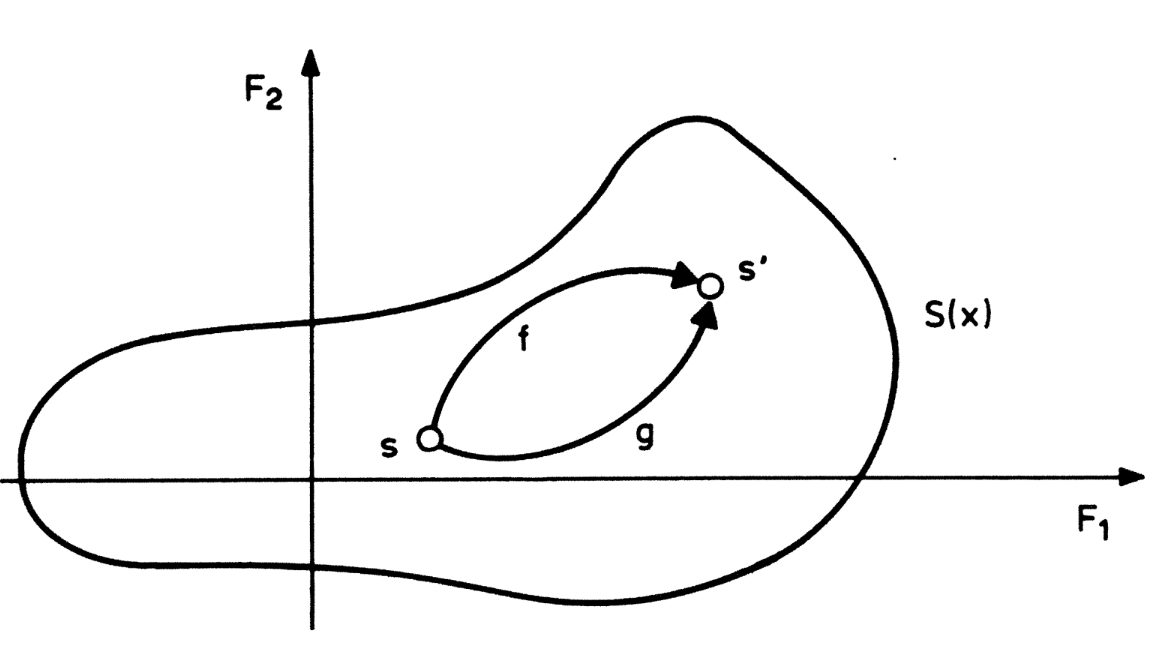
\includegraphics[width=0.9\textwidth]{img/Figura5-5.png}
		\\ \scriptsize Fig. 5.5. Dos procesos diferentes que dan lugar al mismo cambio neto.
	\end{center}
    curva g, donde g $\neq$ f,f, debemos representar los eventos completos, o procesos, mediante
las tripletas ordenadas $\langle s, s^{\prime}, f \rangle$ y $\langle s, s^{\prime}, g \rangle$ respectivamente. 
    Ahora bien, las funciones f y g que aparecen en nuestra ilustración (imaginaria) anterior
    no deben ser arbitrarias: deben ser legales si
    queremos permitir solo eventos legales y descartar todos los imposibles. En otras palabras, f y g deben ser leyes que posea la cosa
    x en cuestión o transformaciones del espacio de estados legales $Sl(X)$ compatibles
    con esas leyes. (Las funciones no tienen por qué ser funciones legales: pueden
    representar leyes objetivas junto con restricciones y circunstancias, como
    condiciones iniciales y condiciones límite, o pueden ser cambios de
    representación que dejen inalteradas todas las leyes de la cosa). Esto
    sugiere hacer
    
    DEFINICION 5.8 $S_{\mathbb{L}}(x)$ ser un espacio de estados legítimo para una cosa x. Entonces, la
familia de transformaciones legítimas del espacio de estados en sí mismo es el conjunto de
funciones
    \begin{center}
        $G_{\mathcal{L}}(x)=\{g \text{ is a function } |g:S_{\mathcal{L}}(x)\rightarrow S_{\mathcal{L}}(x)
        \text{ \& } g \text{ is compatible with the laws of } x\}$.
    \end{center}

    Claramente, la transformación de identidad $i_{S}: S_{\mathcal{L}}(x)\rightarrow S_{\mathcal{L}}(x)$, donde $i_{S}(s)=s$ por cada $s\in S_{\mathcal{L}}(x)$, es miembro fundador de $G_{\mathcal{L}}(x)$. No representa ningún cambio y puede componerse con cualquier transformación no trivial dada.

Cada una de estas transformaciones no triviales $g \in G_L(x)$, donde $g \neq i_S$, ayuda a representar una característica del cambio total experimentado por x, por ejemplo, su cambio de lugar, de población o de aglomeración. Dado que los cambios reales son multifacéticos, deben representarse con la ayuda de una serie de transformaciones diferentes que se combinan para formar el cambio total. Así, un evento termoeléctrico puede considerarse como la composición de un evento térmico y un evento eléctrico, pero no en el sentido de «composición».


    cubierta por la operación binaria * introducida en la sección 2.2. (La acepción
    de «composición» empleada en la presente sección se entiende mejor

    si se tiene en cuenta que $G_L(x)$ is a proper subset of $S_L(x)^{S_L(x)}$, i.e. the family of all the functions on $S_L(x)$ -- not just those representing lawful changes. But the wider set has the monoid structure, since the composition of any two transformations of $S_L(x)$ is a third transformation of the same set, and the latter includes the identity transformation.)
    
        Ahora pasemos al concepto de interés:
    
    \textbf{PRINCIPIO 5.3} Deja $S_L(x)$ ser un espacio de estado legítimo para una cosa $x$, y deja $G_L(x)$ ser la familia de transformaciones legales del espacio de estados    en sí mismo. Entonces, un evento (o proceso) legal con puntos finales $s$ and $s'$, donde $s, s' \in S_L(x)$, es representable como un triple $\langle s, s', g   \rangle$, donde $g \in G_L(x)$ y $s' = g(s)$.

    A esto lo llamamos el \emph{representación funcional del cambio}. Claramente, subsumirá la representación del par ordenado, que se obtiene cuando la transformación $g$ Claramente, subsumirá la representación del par ordenado, que se obtiene cuando la transformación

    ConConsideremos el caso paradigmático del modelo clásico de una partícula. El   estado dinámico instantáneo de tal cosa (modelo) moviéndose en una línea viene  dado por los valores instantáneos de la posición $q$ y el momento $p$ de la    partícula, considerados como variables independientes. El espacio de estados nomológico (llamado \emph{espacio de fase}) de tal cosa es un subconjunto del plano cartesiano. $\mathbb{R}^2$. La transformación que representa el movimiento puede calcularse siempre que se conozcan o se supongan $(a)$ las ecuaciones de movimiento y $(b)$ las fuerzas y restricciones que actúan sobre la partícula. Supongamos, para fijar ideas, que la fuerza que actúa sobre la partícula es elástica. En este caso, nuestro objeto es un oscilador lineal y sus leyes son las ecuaciones canónicas (o de Hamilton), que en este caso particular se reducen a
    \[
    \dot{q} = p/m, \quad \dot{p} = -kq,
    \]
    donde $m$ es la masa de la partícula y $k$ la constante elástica. Luego    llamando $q(t)=q$, $q(t+h)=q'$, donde $h \in \mathbb{R}^+$, y de manera similar para el momento, y expandiendo q' y p' en series de potencias, se obtiene

    \[
    \begin{aligned}
    q' &= q \cos ah + a^{-1}p \sin ah \\
    p' &= p \cos ah - aq \sin ah
    \end{aligned}
    , \text{ with } a = (k/m)^{1/2}.
    \]

    El valor $q'$ de la coordenada de posición en el momento $t$ + $h$ es entonces una función de los valores anteriores tanto de la posición como del momento, y
    lo mismo ocurre con el valor del momento $p'$. Una transformación que representa este cambio (movimiento) se denomina transformación canónica, o una transformación
    que satisface las ecuaciones canónicas del movimiento. Esta transformación,
    para un valor dado del desplazamiento temporal $h$, es una aplicación g:
    
    $\mathbb{R}^2 \to \mathbb{R}^2$ de tal manera que $g(q, p) = \langle q', p' \rangle$ como arriba. (Hay dos funciones involucradas, pero pueden considerarse simplemente como dos componentes de $g$.) La transformación puede considerarse como una rotación en el espacio de estados, donde los ejes cartesianos son ahora $x = a^{-1}p$ y $y=q$, y el ángulo de rotación $\alpha = ah$. y el ángulo de rotación. Esta transformación, lejos de ser arbitraria, está limitada por las leyes del movimiento. El efecto neto de esta restricción es que la elipse $p^2/a^2 + q^2 = 1$ se transforma en la elipse $p'^2/a^2 + q'^2 = 1$ en lugar de convertirse en una curva de otro tipo.

    A menos que el espacio de estados sea unidimensional, el cambio estará   representado por más de una función definida en el espacio de estados. Así, en el ejemplo anterior, la función de transformación resultó tener dos componentes, $u$ y $v$, de tal manera que $q' = u(q, p)$ y $p' = v(q, p)$. pero $u$  y $v$ son, como se ha señalado anteriormente, los dos componentes de una sola función $g$ cartografía $S(x)$ en sí mismo y satisfaciendo las ecuaciones de movimiento.
    
    \subsection{El espacio de los acontecimientos legales}

    In Sec. 2.2 Hemos caracterizado el espacio de eventos netos concebibles. Ahora pasamos a caracterizar el espacio de eventos realmente posibles. (i.e. lawful) eventos, teniendo en cuenta todos los estados intermedios entre los puntos finales que definen los eventos de red. Principio de recuerdo 5.3 en relación con la representación funcional de un proceso completo —no solo sus puntos finales— como un triple ordenado. $\langle s, s', g \rangle$. La recopilación de todos estos triples para una transformación fija. $g$ puede considerarse como un conjunto de pares ordenados y un subconjunto del espacio $E(x)$ de acontecimientos concebibles. Representa la totalidad de los cambios de tipo $g$ que ocurre en o a algo $x$. Y el espacio total de eventos para una cosa determinada es la colección de todos esos espacios de eventos parciales. Más explícitamente, proponemos

    \textbf{DEFINICION 5.9} Deja $S_L(x)$ ser un espacio de estado legítimo para una cosa $x$, y dejar $G_L(x) \subseteq S_L(x)^{S_L(x)}$ ser la familia de transformaciones legales de $S_L(x)$. Entonces
    (i) el $g$-transformaciones legales (o conjunto de\textit{cambios de tipo g})   for $x$, or \textit{espacio de sucesos g-legítimos} en $x$, es el conjunto de     pares ordenados de estados
    $E_g(x) = \{ \langle s, s' \rangle | s, s' \in S_L(x) \times S_L(x) | s' = g    (s) \ \& \ g \in G_L(x) \}$;
    (ii) el \textit{totalidad de las transformaciones legales} de $x$, o \textit    {espacio de eventos legales} (en todos los aspectos) en $x$, es la unión de     todos los espacios parciales de eventos:
    \[ E(x) = \bigcup_{g \in G_L(x)} E_g(x). \]

    (Podríamos haber definido $E_L(x)$ como la familia de todos $E_g(x)$'s, pero    entonces un evento singular perteneciente a cualquiera de los últimos no   pertenecería a los primeros.)

    Relajemos ahora la condición de que las transformaciones del espacio de     estados legales sean ellas mismas legales, y consideremos el espacio de     eventos concebibles. Ahora estamos en condiciones de generalizar el resultado   obtenido en la sección 2.2 relativo a los eventos netos. Consideremos los     eventos $\langle s, s', g \rangle$ y $\langle s', s'', h \rangle$, donde $s,    s', s'' \in S_L(x)$, y $g, h \in G(x) = S_L(x)^{S_L(x)}$. Es decir,    consideramos dos procesos concebibles que ocurren en una misma cosa. Debido a  las transformaciones $g$ y $h$ Es decir, consideramos dos procesos concebibles   que ocurren en una misma cosa. Debido a las transformaciones 
    \[ s \xrightarrow{g} s' \xrightarrow{h} s'' \]
    para producir el cambio neto $\langle s, s'', h \circ g \rangle$, donde     '$\circ$' significa composición de funciones. En el caso particular en que  $h=i_S$ (identity) obtenemos
    \[ s \xrightarrow{g} s' \xrightarrow{i_S} s' \]
    lo que se reduce a $\langle s, s', g \rangle$. Esto demuestra que el espacio    de los acontecimientos concebibles es una categoría. Más concretamente, lo     hemos demostrado con total generalidad.

    \textbf{TEOREMA 5.1} Deja $S_L(x)$ ser un espacio de estado legítimo para una   cosa $x$, and $G(x)=S_L(x)^{S_L(x)}$ la totalidad de (legal e ilegal)     transformaciones de $S_L(x)$. Además, dejemos que '$\circ$' designar la     composición de transformaciones (funciones) en $G$. Luego el triple $\mathcal   {C} = \langle S_L(x), G(x), \circ \rangle$, llamado el \textit{espacio     concebible de x}, es una categoría. Los objetos de esta categoría son todos     los estados. $s \in S_L(x)$ de la cosa, los morfismos, todas las    transformaciones $s \xrightarrow{g} s'$ con $g \in G(x)$ y $s' = g(s)$, y the  identidades las funciones $s \xrightarrow{i_S} s$.

    Este resultado (obtenido con la ayuda de Arturo Sangalli) no es muy     importante porque se refiere a la estructura del espacio de los acontecimientos concebibles  y no a la de los acontecimientos legales. Sin embargo, muestra la estructura en la que   el espacio de los acontecimientos legales $\mathscr{E}_L(x) = \langle S_L(x), G_L(x), \circ  \rangle$ está integrado. Además, nos enseña cómo componer eventos completos en lugar de solo eventos de red. De hecho, hemos aprendido que la composición de eventos se lleva a cabo tal y como indica

    \textbf{DEFINICION 5.10} Deja $S_L(x)$ ser un espacio de estado para una cosa $x$, Y   $G_L(x)$ el conjunto correspondiente de transformaciones legales de $S_L(x)$. Further,  llamada $e=\langle s, s', g \rangle$ and $e' = \langle s', s'', h \rangle$ dos eventos en el espacio legal para eventos $E_L(x)$ definido por $S_L(x)$ Y $G_L(x)$.  Entonces $e$ Y $e'$ \textit{compose} en el orden indicado para formar un tercer evento $e''$ si y solo si el final del primero coincide con el comienzo del segundo y si las dos transformaciones se componen para formar una tercera transformación legítima. Si la composición tiene lugar, entonces se dice que el primer evento\textit{preceder} el segundo. En símbolos:
    (i)
    \[
    \langle s, s', g \rangle * \langle s', s'', h \rangle =
    \begin{cases}
        \langle s, s'', h \circ g \rangle & \text{if } s' = s'' \text{ \& } h   \circ g \in G_L(x) \\
        \text{undefined} & \text{otherwise}
    \end{cases}
    \]
    (ii) $e < e' =_{df} e * e' \in E_L(x)$.

    Y ahora algunas ilustraciones atrasadas.

    \textbf{Ejemplo 1} Supongamos que se trata de un sistema conservativo con $n$ componentes.  Su espacio de estados clásico es el espacio cartesiano de dimensión $6n$ generado por     la función de estado cuyos componentes son las $3n$ coordenadas de posición generalizadas   y los $3n$ momentos. El espacio de sucesos está incluido en el conjunto de   gráficos de las transformaciones canónicas o de contacto, que son aquellas   transformaciones del espacio de estados (fase) que dejan invariantes las leyes del movimiento . Para más detalles sobre el caso más simple, véase el ejemplo de la sección 2.3.
    \textbf{Ejemplo 2} El espacio de estados de un sistema cuántico-mecánico es un espacio de Hilbert, es decir, un conjunto determinado de funciones. El operador $T = \exp(iHt/\hbar)$ definido en este espacio, es decir, $T: S \to S$, permite representar los cambios en los estados del sistema. Por lo tanto, si $Q(t_0)$ representa el valor de una propiedad $Q$    del sistema en el momento $t_0$, entonces su valor en el momento $t$ es $Q(t) = TQ(t_0)T^   {-1}$.
    \textbf{Ejemplo 3} Algunos o incluso todos los componentes de la función de estado  para una cosa podrían ser variables aleatorias. Entonces, el espacio de estado correspondiente   sería un espacio de estado probabilístico (cap. 4, sec. 4.2). Las leyes del cambio, o  al menos algunas de ellas, no se referirían a los estados de manera directa, sino   más bien a sus probabilidades o, mejor dicho, a las probabilidades de las diversas  transiciones de estado posibles (legítimas). Estas probabilidades son condicionales.  Consideremos el caso simple de un espacio de estado con un número finito de puntos, cada uno de los cuales tiene una probabilidad definida. Cada estado final $s_f$ puede surgir (originarse) a partir de cualquier otro estado $s_i$ con una probabilidad definida $\Pr(s_f|s_i)$, que por supuesto puede ser nula para algunos pares de estados. Para un $i$ fijo, todas estas probabilidades suman la unidad. La probabilidad total de que se actualice un estado $s_f$ es
\[
\Pr(s_f) = \sum_i \Pr(s_i) \cdot \Pr(s_f|s_i).
\]

\subsection*{2.5. Seguimiento de los estados cambiantes}
Mientras que algunas propiedades de una cosa, como su composición, son invariables o absolutas, otras, como su energía, dependen del marco o son relativas. Dado que todas las cosas poseen energía, los estados de todas las cosas son relativos: recuerde el capítulo 3, sección 2.8. Y como los estados son relativos, también lo son los acontecimientos. Es cierto que acontecimientos como encender un interruptor o besar parecen absolutos. Pero esto se debe únicamente a que, al pensar en ellos, nos centramos en lo que parece típico, dejando de lado una serie de características que dependen del marco, como la ubicación y la velocidad de la(s) cosa(s) en la(s) que se producen los acontecimientos. Una descripción razonablemente completa de un acontecimiento requiere la determinación de una serie de rasgos, la mayoría de los cuales están destinados a ser relativos más que absolutos. Por lo tanto,

\textbf{RULE 6.1} Referir cada función de estado es decir, cada espacio de estado y cada espacio de eventos— a algún elemento estándar (marco de referencia) u otro.

La referencia explícita a los estándares no solo sirve como recordatorio de que el cambio es relativo: también puede utilizarse para etiquetar estados y realizar un seguimiento de ellos de una forma más precisa que hasta ahora. De hecho, este es el objetivo de la Definición 3.14: nos permite identificar los estados de las cosas en términos de estados de referencia o estados de un estándar. Recordemos cómo se hizo esto y mejoremos esa parametrización.
Sea $S(f)$ un espacio de estados de un marco de referencia $f$ para un objeto $x$ con espacio de estados $S(x)$. Además, supongamos que el dominio de la función de estado $F$ que abarca $S(x)$, lejos de no estar relacionado con el marco de referencia, es igual a la colección $S(f)$ de estados de referencia. Es decir, establezcamos $F: S(f) \to S(x)$, de modo que cada estado de referencia $t \in S(f)$ se empareje con un único estado de cosa $s=F(t) = \langle F_i(t)| 1 \le i \le n \rangle$, donde $n$ es el número de propiedades representadas por $F$. La función de estado $F$ es ahora la lista de propiedades de la cosa $x$ \textit{relativa a} (o parametrizada por) los estados del marco de referencia $f$. Dado cualquier estado de referencia $t$, $F$ elige el estado de cosa correspondiente $F(t)$. Y una sustitución de puntos, cada uno de los cuales tiene una probabilidad definida. Cada estado final $s_f$ puede surgir (originarse) de cualquier otro estado $s_i$ con una probabilidad definida $\Pr(s_f|s_i)$, que por supuesto puede ser nula para algunos pares de estados. Para un $i$ fijo, todas estas probabilidades suman la unidad. La probabilidad total de que se actualice un estado $s_f$ es
\[
\Pr(s_f) = \sum_i \Pr(s_i) \cdot \Pr(s_f|s_i).
\]

\subsection*{2.5. Seguimiento de los estados cambiantes}

Mientras que algunas propiedades de una cosa, como su composición, son invariables o absolutas, otras, como su energía, dependen del marco o son relativas. Dado que todas las cosas poseen energía, los estados de todas las cosas son relativos: recuerde el capítulo 3, sección 2.8. Y como los estados son relativos, también lo son los acontecimientos. Es cierto que acontecimientos como encender un interruptor o besar parecen absolutos. Pero esto se debe únicamente a que, al pensar en ellos, nos centramos en lo que parece típico, dejando de lado una serie de características que dependen del marco, como la ubicación y la velocidad de la(s) cosa(s) en la(s) que se producen los acontecimientos. Una descripción razonablemente completa de un acontecimiento requiere la determinación de una serie de rasgos, la mayoría de los cuales están destinados a ser relativos más que absolutos. Por lo tanto.

\textbf{RULE 6.1} Referir cada función de estado es decir, cada espacio de estado y cada espacio de eventos— a algún elemento estándar (marco de referencia) u otro.

La referencia explícita a los estándares no solo sirve como recordatorio de que el cambio es relativo: también puede utilizarse para etiquetar estados y realizar un seguimiento de ellos de una forma más precisa que hasta ahora. De hecho, este es el objetivo de la Definición 3.14: nos permite identificar los estados de las cosas en términos de estados de referencia o estados de un estándar. Recordemos cómo se hizo esto y mejoremos esa parametrización.

Sea $S(f)$ un espacio de estados de un marco de referencia $f$ para un objeto $x$ con espacio de estados $S(x)$. Además, supongamos que el dominio de la función de estado $F$ que abarca $S(x)$, lejos de no estar relacionado con el marco de referencia, es igual a la colección $S(f)$ de estados de referencia. Es decir, establezcamos $F: S(f) \to S(x)$, de modo que cada estado de referencia $t \in S(f)$ se empareje con un único estado de cosa $s=F(t) = \langle F_i(t)| 1 \le i \le n \rangle$, donde $n$ es el número de propiedades representadas por $F$. La función de estado $F$ es ahora la lista de propiedades de la cosa $x$ \textit{relativa a} (o parametrizada por) los estados del marco de referencia $f$. Dado cualquier estado de referencia $t$, $F$ elige el estado de cosa correspondiente $F(t)$. Y una sustitución de
puntos, cada uno de los cuales tiene una probabilidad definida. Cada estado final
 $s_f$ puede surgir (tener su origen) en cualquier otro estado $s_i$ con una probabilidad definida $\Pr(s_f|s_i)$, que, por supuesto, puede ser nula para algunos pares de estados. Para un $i$ fijo, todas estas probabilidades suman la unidad. La probabilidad total de que se actualice el estado $s_f$ es
\[
\Pr(s_f) = \sum_i \Pr(s_i) \cdot \Pr(s_f|s_i).
\]

\subsection*{Seguimiento de los estados cambiantes}

Mientras que algunas propiedades de una cosa, como su composición, son invariables o absolutas, otras, como su energía, son
dependientes o relativas. Dado que todo posee energía, los estados de todo son relativos: recuerde el capítulo 3, sección 2.8. Y como los estados son
relativos, también lo son los acontecimientos. Es cierto que acontecimientos como encender un interruptor o besar
parecen absolutos. Pero esto es solo porque al pensar en ellos nos centramos en lo que parece típico, dejando de lado una serie de características que dependen del marco, como la ubicación y la velocidad de la(s) cosa(s) en la(s) que ocurren los eventos. Una descripción razonablemente completa de un evento requiere la determinación de una serie de rasgos, la mayoría de los cuales están destinados a ser relativos en lugar de absolutos. Por lo tanto

\textbf{RULE 6.1} Remitir todas las funciones estatales - Por lo tanto, cada espacio de estados y cada espacio de eventos se relaciona con algún estándar (marco de referencia) u otro.

La referencia explícita a los estándares no solo sirve como recordatorio de que el cambio es relativo: también puede utilizarse para etiquetar estados y realizar un seguimiento de ellos de una forma más precisa que hasta ahora. De hecho, este es el objetivo de la Definición 3.14: nos permite identificar los estados de las cosas en términos de estados de referencia o estados de un estándar. Recordemos cómo se hizo esto y mejoremos esa parametrización.

Sea $S(f)$ un espacio de estados de un marco de referencia $f$ para un objeto $x$ con espacio de estados $S(x)$. Además, supongamos que el dominio de la función de estado $F$ que abarca $S(x)$, lejos de no estar relacionado con el marco de referencia, es igual a la colección $S(f)$ de estados de referencia. Es decir, establezcamos $F: S(f) \to S(x)$, de modo que cada estado de referencia $t \in S(f)$ se empareje con un único estado de cosa $s=F(t) = \langle F_i(t)| 1 \le i \le n \rangle$, donde $n$ es el número de propiedades representadas por $F$. La función de estado $F$ es ahora la lista de propiedades de la cosa $x$ \textit{relativa a} (o parametrizada por) los estados del marco de referencia $f$. Dado cualquier estado de referencia $t$, $F$ elige el estado de cosa correspondiente $F(t)$. Y una sustitución de

un marco no equivalente $f'$ para el marco $f$ irá acompañado de diferentes valores $F(t')$ de la función de estado.

Los estados de un marco de referencia pueden describirse con diversos grados de precisión. Pero si vamos a utilizarlos para etiquetar o identificar estados de cosas, entonces esa precisión no debe ser inferior a la empleada para describir los estados de las cosas. Ahora bien, en ciencia se suele buscar, y a menudo se alcanza, la máxima precisión, que en este caso consiste en asignar valores reales a las propiedades individuales de las cosas. Es decir, en la mayoría de los casos, cada valor de la función de estado $F_i$ para una cosa dada es igual a un número real $r_n$, de modo que el estado de la cosa en (\textit{relativo a}) $t \in S(f)$ es $F(t) = \langle F_i(t)| 1 \le i \le n \rangle = \langle r_1, r_2, \dots, r_n \rangle$. Un grado tan alto de precisión exige una precisión similar en la descripción de los estados de referencia. Y esa precisión se consigue coordinándolos, es decir, asignándoles valores de coordenadas.

El procedimiento de coordinatización se visualiza mejor interpretando $S(f)$ como un sistema de cuatro ejes cartesianos, de modo que a cada estado de referencia se le asigna un cuádruple de números reales. Es decir, seleccionamos aquellas propiedades de un marco de referencia que pueden representarse en una cuadrícula de cuatro dimensiones, dejando de lado todas las demás propiedades. (Los puntos de la cuadrícula se interpretan finalmente como puntos en el espacio-tiempo). Por último, nos referimos a los estados de las cosas no en relación con los estados de referencia, sino con sus etiquetas numéricas. - Cuando decimos $'X$ estaba soñando en la esquina de la calle en 7:00 p.m.'. Es decir, emparejamos cada estado de cosa con un punto en la cuadrícula de referencia.

La coordinatización de los estados de referencia se efectúa mediante una correspondencia uno a uno. $k: \mathbb{R}^4 \to S(f)$ entre cuádruples ordenadas de números reales y estados de referencia. La composición $\lambda = F \circ k$ de la función de coordinatización con la función de estado coincide con cada punto $r = \langle t, x, y, z \rangle$ en la cuadrícula de referencia con un estado de cosa $s$, i.e. $r \xrightarrow{k} t \xrightarrow{F} s$, como se muestra en la figura 5.6 y en el diagrama conmutativo de la página siguiente.

Ahora, la cuadrícula de referencia está parcialmente ordenada. De hecho, si $r$ y $s$ son cuádruples de números reales, entonces $r \le s$ si y solo si cada componente o coordenada de $r$ es menor que la coordenada correspondiente de $s$. Es decir,
\[
\langle r_1, r_2, r_3, r_4 \rangle \le \langle s_1, s_2, s_3, s_4 \rangle \text{ iff } r_i \le s_i \text{ for all } i=1, 2, 3, 4.
\]
En consecuencia $\langle S(f), \le \rangle$ es un conjunto parcialmente ordenado. Este orden no está conectado: no todos los pares de estados de referencia están relacionados por $\le$: véase la figura 5.7. Y se impone el mismo tipo de orden, a través de $F$, en el plató $S(x)$ de cosa.

	\begin{center}
		\includegraphics[width=0.9\textwidth]{img/Figura5-6.png}
		\\ \scriptsize Fig. 5.6. Coordinatización de estados. Cada estado de referencia $t \in S(f)$ se asigna como máximo un estado de cosa $s \in S(x) \subseteq \mathbb{R}^n$ y está representado por un cuádruple de números reales $r \in \mathbb{R}^4$.
	\end{center}

	\begin{center}
		\includegraphics[width=0.9\textwidth]{img/Figura5-7.png}
		\\ \scriptsize Fig. 5.7. El estado $s$ precede a todos los demás en la región sombreada, pero a ninguno fuera de esta.
	\end{center}

    estados incluso si $F$ dno toma valores en $\mathbb{R}^n$ - como cuando se dice que un mamífero pasa por cuatro etapas de desarrollo.

    Las consideraciones anteriores pueden resumirse en

    \textbf{DEFINITION 5.11} deja $f$ ser un marco de referencia para algo $x$ y deja $S(f)$ y $S(x)$ sean los respectivos espacios de estados. Además, supongamos que $S(f)$ es

    recorrido por una función de estado de cuatro componentes, mientras que $S(x)$ es explorado por una función de estado de $n$-componentes $F$. Entonces, una \textit{coordenadización de los estados} tanto de $x$ como de $f$ es una correspondencia biunívoca $k: \mathbb{R}^4 \to S(f)$ tal que
(i) $k$ asigna a cada estado de referencia $s \in S(f)$ una cuádrupla de números reales $r$ - como consecuencia de lo cual cada estado del ente $s \in S(x)$ se identifica como la $n$-tupla $s = (F \circ k)(r)$;
(ii) $k$ preserva el orden, es decir, el orden parcial de $\mathbb{R}^4$ induce a través de $k$ el ordenamiento parcial de los estados de referencia, lo que a su vez ordena los estados del ente: para todo $t_1, t_2 \in S(f)$,
\begin{quote}
    si $r_1 \le r_2$ entonces $k(r_1) \le k(r_2) \text{ y } F(t_1) \le F(t_2)$,
    donde \quad $t_i = k(r_i)$.
\end{quote}
En otras palabras, una coordenadización de estados es una función que preserva el orden, etiquetando y ordenando los estados del ente a través de los estados de referencia:
\[
\langle\mathbb{R}^4, \le\rangle \xrightarrow{k} \langle S(f), \le\rangle \xrightarrow{F} \langle S(x), \le\rangle.
\]
A medida que el marco de referencia pasa de un estado a otro, también lo hace el ente: los estados sucesivos de un ente pueden entonces ser asociados y, por lo tanto, identificados por (no \textit{con}) los estados sucesivos del estándar. Y a su vez, el ordenamiento de los estados induce un ordenamiento de los eventos (en el mismo ente y relativo al mismo marco). Por consiguiente, podemos establecer

\textbf{DEFINICIÓN 5.12} Sean $s, s', s'', s'''$ cuatro estados de un ente dado relativos a un cierto marco de referencia, tal que los dos primeros forman un evento neto $e = \langle s, s' \rangle$ y los dos últimos otro evento $e'=\langle s'', s''' \rangle$. Entonces
(i) $e \le e' =_{df} s \le s'' \text{ y } s' \le s'''$.
(ii) $e \sim e' =_{df} e \le e' \text{ y } e' \le e$.
La relación $\le$ de orden de eventos es reflexiva; dos eventos son congruentes si y solo si sus estados iniciales y finales correspondientes son congruentes, es decir,
\[
e \sim e' =_{df} s \sim s'' \text{ y } s' \sim s'''.
\]
Es claro también que $\le$ es antisimétrica y transitiva. Por lo tanto, $\le$ es un orden parcial - a diferencia de la relación introducida en la Definición 5.7, que era solo un orden parcial estricto. Por lo tanto, en lugar del Corolario 5.5 tenemos

\textbf{COROLARIO 5.6} Para todo ente $x$ y relativo a cualquier marco de referencia dado, $\langle E(x), \le \rangle$ es un conjunto parcialmente ordenado.

\end{justifying}
